\documentclass[
  DIV=15,
  bibliography=totoc,     % Literatur im Inhaltsverzeichnis
  captions=tableheading,  % Tabellenüberschriften
  titlepage=firstiscover, % Titelseite ist Deckblatt
]{scrartcl}

% Paket float verbessern
\usepackage{scrhack}

% Warnung, falls nochmal kompiliert werden muss
\usepackage[aux]{rerunfilecheck}

% deutsche Spracheinstellungen
\usepackage{polyglossia}
\setmainlanguage{german}

% unverzichtbare Mathe-Befehle
\usepackage{amsmath}
% viele Mathe-Symbole
\usepackage{amssymb}
% Erweiterungen für amsmath
\usepackage{mathtools}

% Fonteinstellungen
\usepackage{fontspec}
% Latin Modern Fonts werden automatisch geladen

\usepackage[
  math-style=ISO,    % ┐
  bold-style=ISO,    % │
  sans-style=italic, % │ ISO-Standard folgen
  nabla=upright,     % │
  partial=upright,   % ┘
  warnings-off={           % ┐
    mathtools-colon,       % │ unnötige Warnungen ausschalten
    mathtools-overbracket, % │
  },                       % ┘
]{unicode-math}

% traditionelle Fonts für Mathematik
\setmathfont{Latin Modern Math}
\setmathfont{XITS Math}[range={scr, bfscr}]
\setmathfont{XITS Math}[range={cal, bfcal}, StylisticSet=1]

% Zahlen und Einheiten
\usepackage[
  locale=DE,                 % deutsche Einstellungen
  separate-uncertainty=true, % immer Fehler mit \pm
  per-mode=reciprocal,       % ^-1 für inverse Einheiten
  % output-decimal-marker=.,   % . statt , für Dezimalzahlen
]{siunitx}

% chemische Formeln
\usepackage[
  version=4,
  math-greek=default, % ┐ mit unicode-math zusammenarbeiten
  text-greek=default, % ┘
]{mhchem}

% richtige Anführungszeichen
\usepackage[autostyle]{csquotes}

% schöne Brüche im Text
\usepackage{xfrac}

% Standardplatzierung für Floats einstellen
\usepackage{float}
\floatplacement{figure}{htbp}
\floatplacement{table}{htbp}

% Floats innerhalb einer Section halten
\usepackage[
  section, % Floats innerhalb der Section halten
  below,   % unterhalb der Section aber auf der selben Seite ist ok
]{placeins}

% Seite drehen für breite Tabellen
\usepackage{pdflscape}

% Captions schöner machen.
\usepackage[
  labelfont=bf,        % Tabelle x: Abbildung y: ist jetzt fett
  font=small,          % Schrift etwas kleiner als Dokument
  width=0.9\textwidth, % maximale Breite einer Caption schmaler
]{caption}
% subfigure, subtable, subref
\usepackage{subcaption}

% Grafiken können eingebunden werden
\usepackage{graphicx}
% größere Variation von Dateinamen möglich
\usepackage{grffile}

% schöne Tabellen
\usepackage{booktabs}

% Verbesserungen am Schriftbild
\usepackage{microtype}

% Literaturverzeichnis
\usepackage[
  backend=biber,
]{biblatex}
% Quellendatenbank
\addbibresource{lit.bib}
\addbibresource{programme.bib}

% Hyperlinks im Dokument
\usepackage[
  unicode,        % Unicode in PDF-Attributen erlauben
  pdfusetitle,    % Titel, Autoren und Datum als PDF-Attribute
  pdfcreator={},  % ┐ PDF-Attribute säubern
  pdfproducer={}, % ┘
]{hyperref}
% erweiterte Bookmarks im PDF
\usepackage{bookmark}

% Trennung von Wörtern mit Strichen
\usepackage[shortcuts]{extdash}

%(Python-) Code ein binden 
\usepackage{listings}
\usepackage{color}
\definecolor{mygreen}{rgb}{0,0.6,0}
\definecolor{mygray}{rgb}{0.5,0.5,0.5}
\definecolor{mymauve}{rgb}{0.58,0,0.82}

\lstset{ 
  backgroundcolor=\color{white},   % choose the background color; you must add \usepackage{color} or \usepackage{xcolor}; should come as last argument
  basicstyle=\footnotesize,        % the size of the fonts that are used for the code
  breakatwhitespace=false,         % sets if automatic breaks should only happen at whitespace
  breaklines=true,                 % sets automatic line breaking
  captionpos=b,                    % sets the caption-position to bottom
  commentstyle=\color{mygreen},    % comment style
  deletekeywords={...},            % if you want to delete keywords from the given language
  escapeinside={\%*}{*)},          % if you want to add LaTeX within your code
  extendedchars=true,              % lets you use non-ASCII characters; for 8-bits encodings only, does not work with UTF-8
  frame=single,	                   % adds a frame around the code
  keepspaces=true,                 % keeps spaces in text, useful for keeping indentation of code (possibly needs columns=flexible)
  keywordstyle=\color{blue},       % keyword style
%  language=Octave,                 % the language of the code
  morekeywords={*,...},            % if you want to add more keywords to the set
  numbers=left,                    % where to put the line-numbers; possible values are (none, left, right)
  numbersep=5pt,                   % how far the line-numbers are from the code
  numberstyle=\tiny\color{mygray}, % the style that is used for the line-numbers
  rulecolor=\color{black},         % if not set, the frame-color may be changed on line-breaks within not-black text (e.g. comments (green here))
  showspaces=false,                % show spaces everywhere adding particular underscores; it overrides 'showstringspaces'
  showstringspaces=false,          % underline spaces within strings only
  showtabs=false,                  % show tabs within strings adding particular underscores
  stepnumber=1,                    % the step between two line-numbers. If it's 1, each line will be numbered
  stringstyle=\color{mymauve},     % string literal style
  tabsize=2,	                   % sets default tabsize to 2 spaces
  title=\lstname                   % show the filename of files included with \lstinputlisting; also try caption instead of title
}
%\titlehead{
%        \hfill
%        
\includegraphics[height= 1cm]{./pics/tu_logo.jpg}
%        }
%
%\author{
%  Yvonne Kasper%
%  \texorpdfstring{
%    \\
%    \href{mailto:authorA@udo.edu}{yvonne.kasper@udo.edu}
%  }{}%
%  \texorpdfstring{\and}{, }
%  Robert Appel%
%  \texorpdfstring{
%    \\
%    \href{mailto:authorB@udo.edu}{robert.appel@udo.edu}
%  }{}%
%  \texorpdfstring{\and}{, }
%  Julian Schröer%
%  \texorpdfstring{
%    \\
%    \href{mailto:authorB@udo.edu}{julian.schroeer@udo.edu}
%  }{}%
%}
%\publishers{TU Dortmund – Fakultät Physik}

%\subject{Statistische Methoden der Datenanalyse}
%\title{Blatt 1}
%\date{
%  Abgabe: 26.10.2018
%}
\begin{document}

%\maketitle
%\thispagestyle{empty}
%\tableofcontents
%\newpage
%\setcounter{page}{1}
\begin{center}
{\huge SMD-Nikolaus-Übungsblatt (7) } \\
\vspace{1cm}
Abgabe: 06.12.18 \\
\vspace{.5cm}
  Yvonne Kasper
  \texorpdfstring{
    \href{mailto:authorA@udo.edu}{yvonne.kasper@udo.edu}
  }{},\\
  Robert Appel%
  \texorpdfstring{
    \href{mailto:authorB@udo.edu}{robert.appel@udo.edu}
  }{},\\
  Julian Schröer%
  \texorpdfstring{
    \href{mailto:authorB@udo.edu}{julian.schroeer@udo.edu}
  }{}
\end{center}
%\section{Aufgabe1}
\label{sec:Aufgabe1}
\lstinputlisting[language=Python, firstline=15, lastline=21]{plots/plot.py}
\paragraph{Wiederholung der Methoden aus der Vorlesung}
Gegeben:
\begin{equation}
 f(u) = U(0,1) = 
\begin{cases}
1, & 0 \leq x < 1 \\
0, & \text{sonst}
\end{cases}	
\end{equation}
Hier bezeichnet u gleichverteilte Zufallsvariablen mit der Wahrscheinlichkeitsdichte $f(u)$. 
Gesucht: 
\begin{equation}
g(y) \quad \text{mit} \quad y \in [y_{min},y_{max}]	
\end{equation}
Dabei bezeichnet $y$ eine Zufallsvariable mit der Wahrscheinlichkeitsdichte $g(y)$. 
Die Transformation einer Gleichverteilung, um Zufallszahlen aus einer beliebigen Verteilung 
zu generieren ist gegeben durch
\begin{gather}
g(y) \symup{d} = U(0,1)\symup{du} \\
\implies u = \int_{u_{min}} ^{u} U(0,1) \symup{d}u  = G(y) = \int_{y{min}} ^{y} g(y') \symup{d}y' \\
\implies y = G^{-1}(u) \; .
\label{eq:methods}
\end{gather}
Für den Programmierteil dieser Aufgabe wurden die zufälligen Werte wie folgt erstellt.
\lstinputlisting[language=Python, firstline=16, lastline=18]{plots/Aufgabe1.py} 


\subsection{a)}
Mit den zuvor dargestellten Methoden ergibt sich die Funktion
\begin{equation}
y = u \cdot (b-a) + a \; .
\end{equation}
Die dazugehörigen Rechnungen sind in der Abbildung \ref{fig:A1ab} dargestellt.
In der Abbildung \ref{fig:A1abcd} in der oberen linken Ecke findet sich ein Histogramm der 
Funktion (grün). Im selben Histogramm ist die gegebene Gleichverteilung die Werte in 
den Grenzen [0,1] ausgibt gezeigt. In Python wurde die Funktion wie folgt implementiert.

\lstinputlisting[language=Python, firstline=20, lastline=21]{plots/Aufgabe1.py}

\subsection{b)}
Mit den zuvor dargestellten Methoden ergibt sich die Funktion
\begin{equation}
y = - \tau \ln(1-u) \; .	
\end{equation}
Die dazugehörigen Rechnungen sind in der Abbildung \ref{fig:A1ab} dargestellt.
In der Abbildung \ref{fig:A1abcd} in der oberen rechten Ecke findet sich ein Histogramm der 
Funktion (blau).In Python wurde die Funktion wie folgt implementiert.

\lstinputlisting[language=Python, firstline=23, lastline=24]{plots/Aufgabe1.py}


\subsection{c)}
Mit den zuvor dargestellten Methoden ergibt sich die Funktion
\begin{equation}
y = \left( u \cdot \left(b^{1-n} - a^{1-n} \right) + a^{1-n} \right)^{\frac{1}{1-n}} \; .
\end{equation}
Die dazugehörigen Rechnungen sind in der Abbildung \ref{fig:A1cd} dargestellt.
In der Abbildung \ref{fig:A1abcd} in der unteren linken Ecke findet sich ein Histogramm der 
Funktion (blau).In Python wurde die Funktion wie folgt implementiert.

\lstinputlisting[language=Python, firstline=26, lastline=27]{plots/Aufgabe1.py}

\subsection{d)}
Mit den zuvor dargestellten Methoden ergibt sich die Funktion
\begin{equation}
y = \tan ( \pi (u +1 ))
\end{equation}
Die dazugehörigen Rechnungen sind in der Abbildung \ref{fig:A1cd} dargestellt.
In der Abbildung \ref{fig:A1abcd} in der unteren rechten Ecke findet sich ein Histogramm der 
Funktion (blau).In Python wurde die Funktion wie folgt implementiert.

\lstinputlisting[language=Python, firstline=29, lastline=30]{plots/Aufgabe1.py}

\begin{figure}
\begin{subfigure}{.48\textwidth}
  \centering
  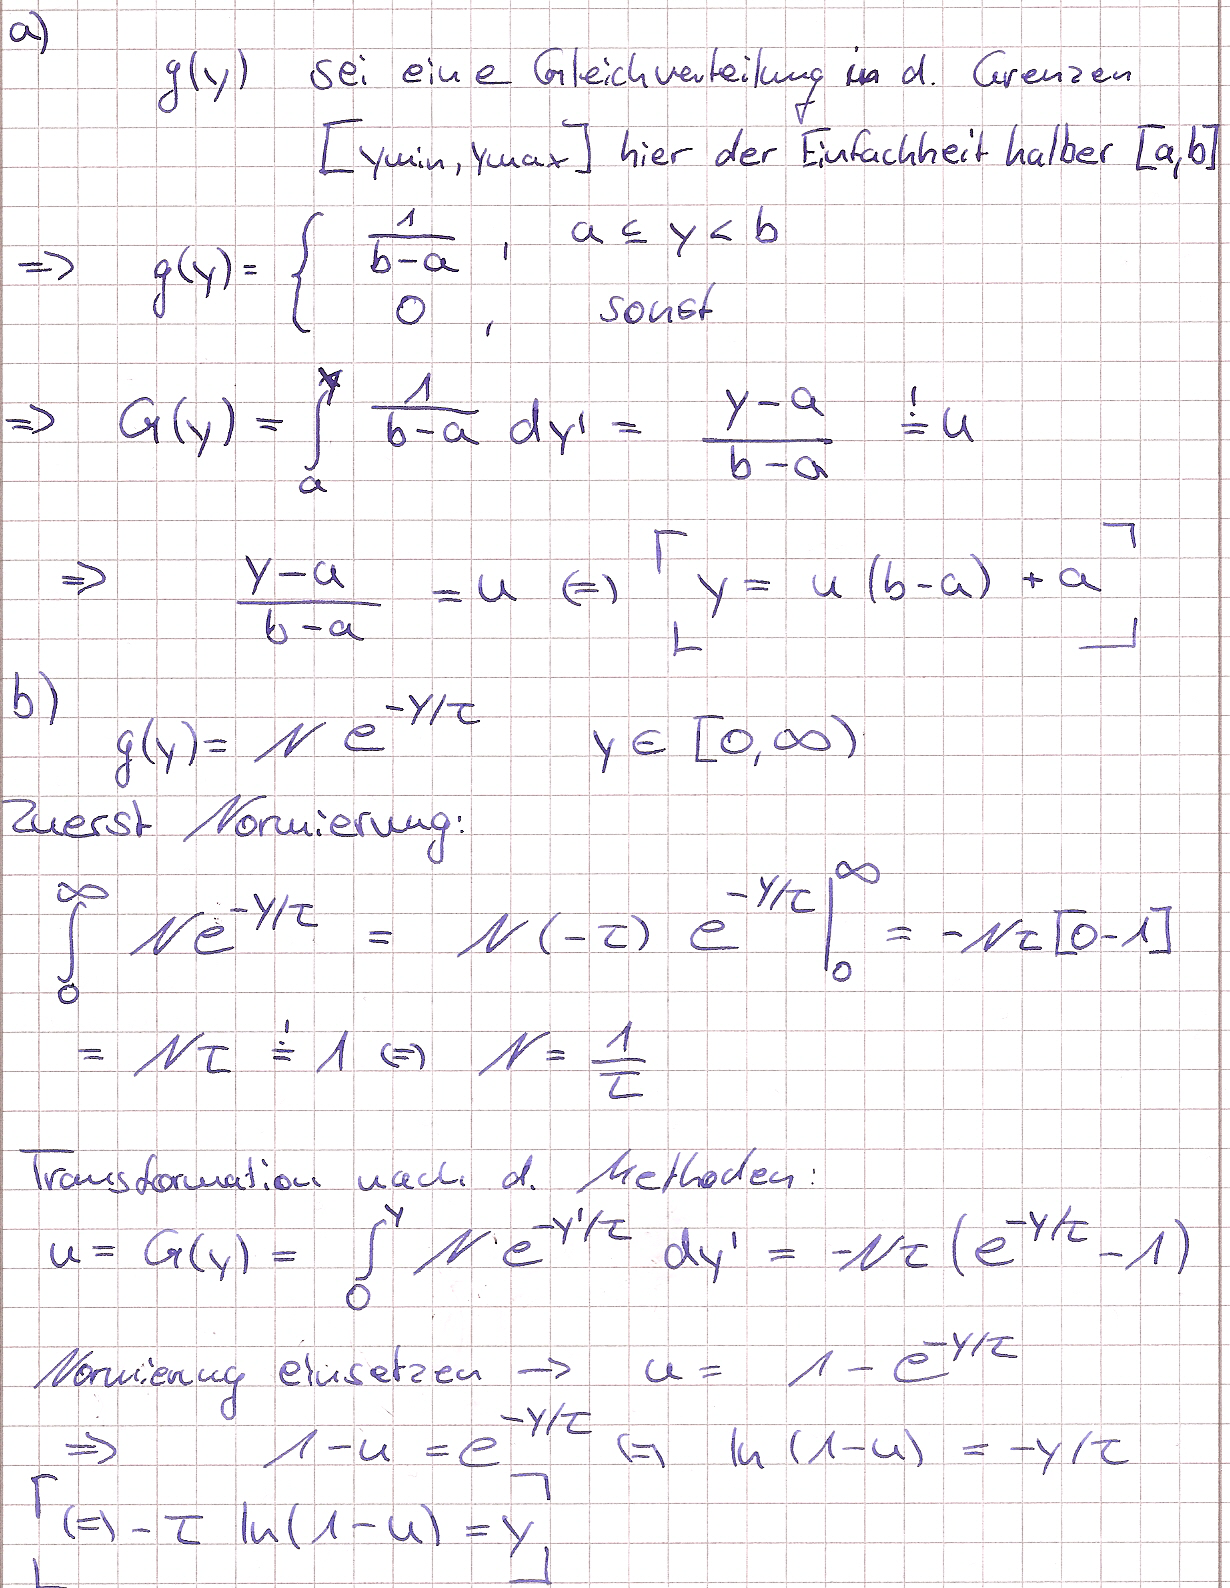
\includegraphics[height = 10cm]{pics/A1ab}
  \caption{a) und b).}
  \label{fig:A1ab}
\end{subfigure}
\begin{subfigure}{.48\textwidth}
  \centering
  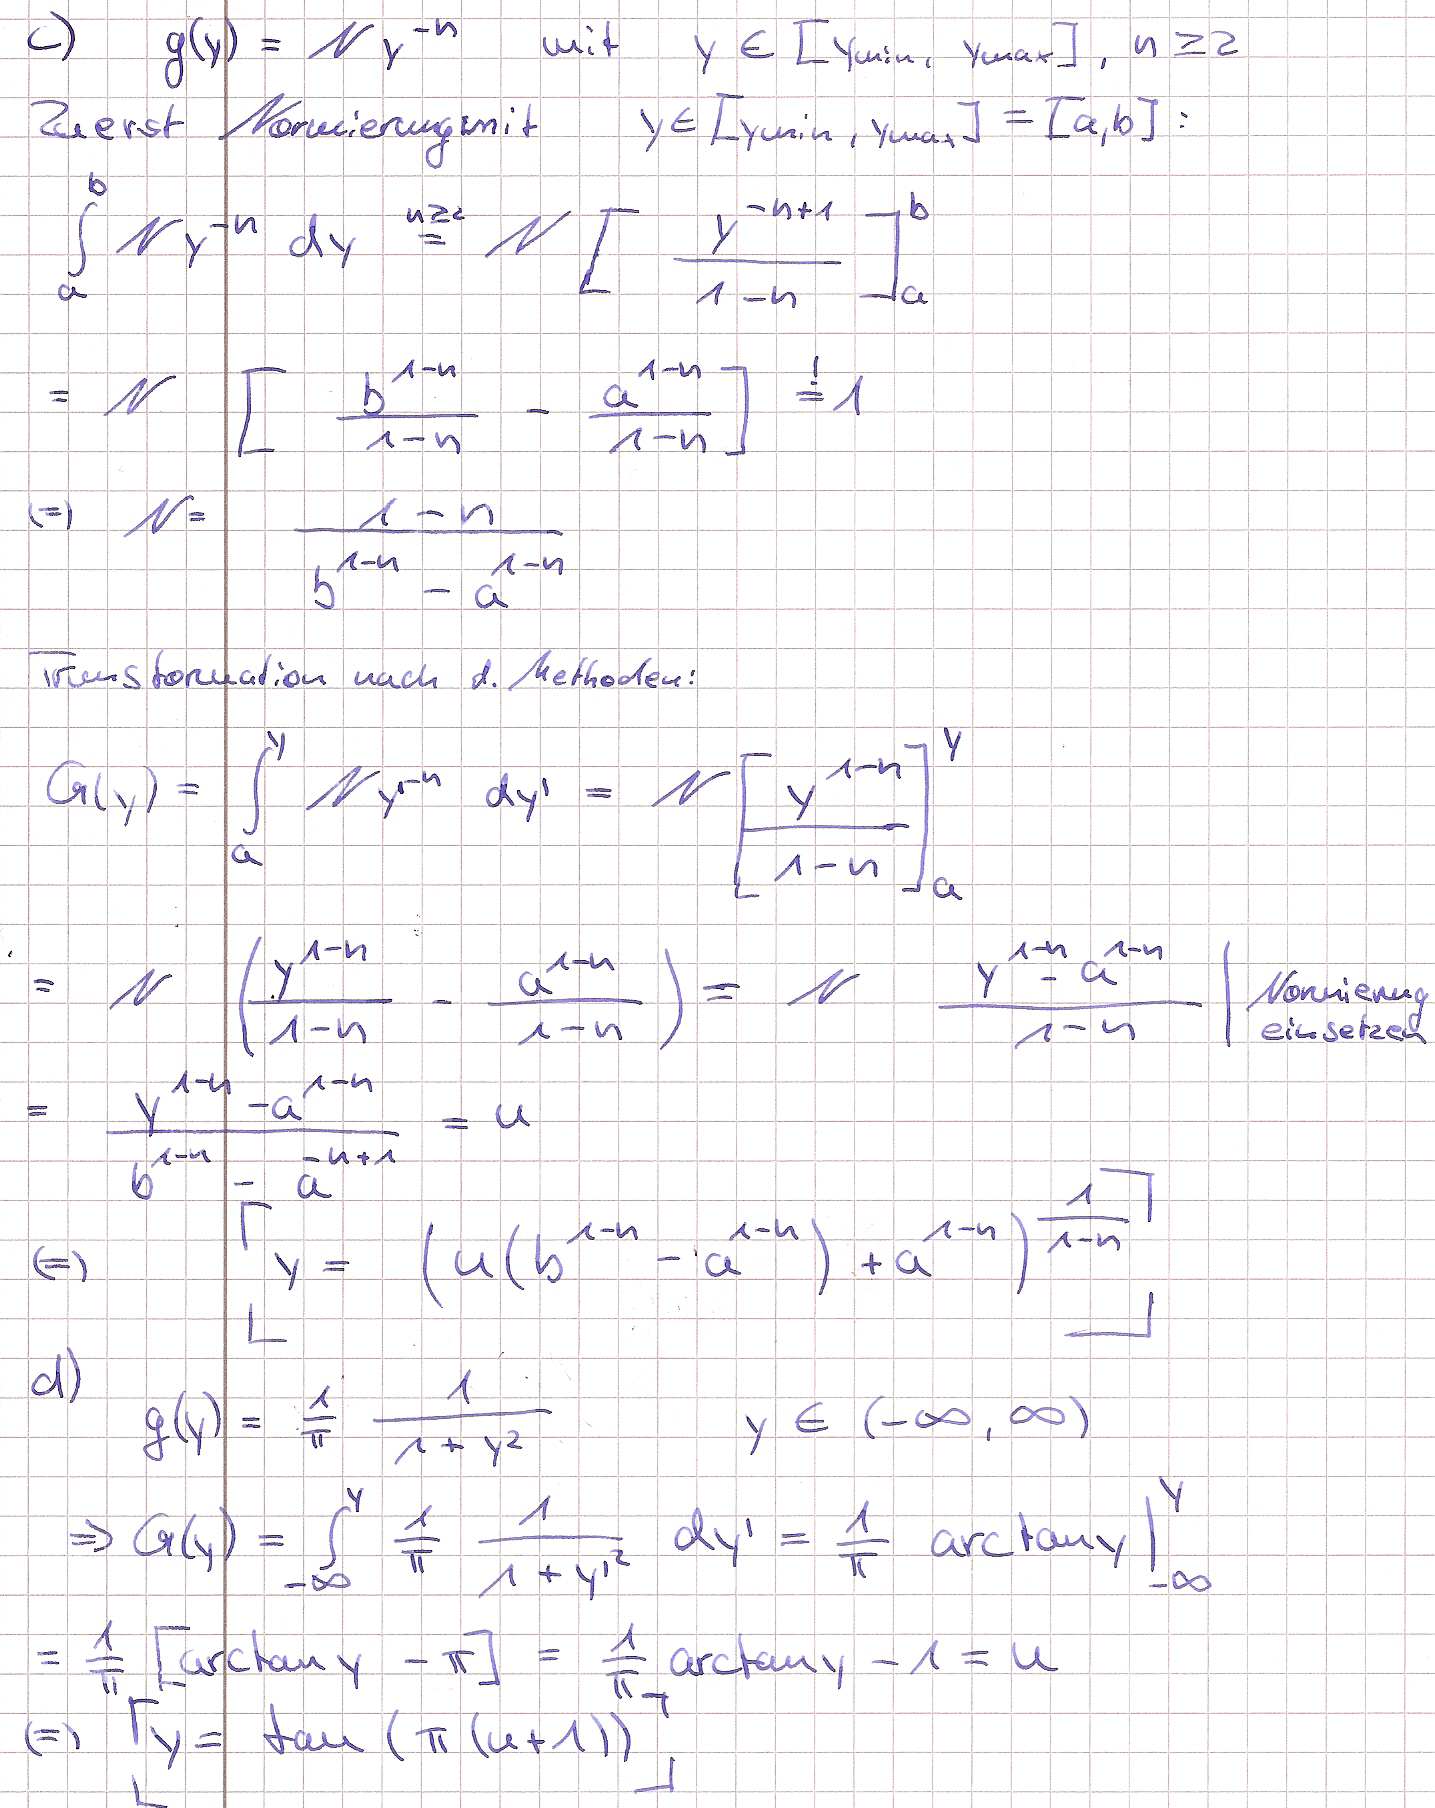
\includegraphics[height = 10cm]{pics/A1cd}
  \caption{c) und d).}
  \label{fig:A1cd}
\end{subfigure}
  \caption{Rechnungen zu Aufgabe1}
  \label{fig:A1rech}
\end{figure}

\begin{figure}
  \centering
  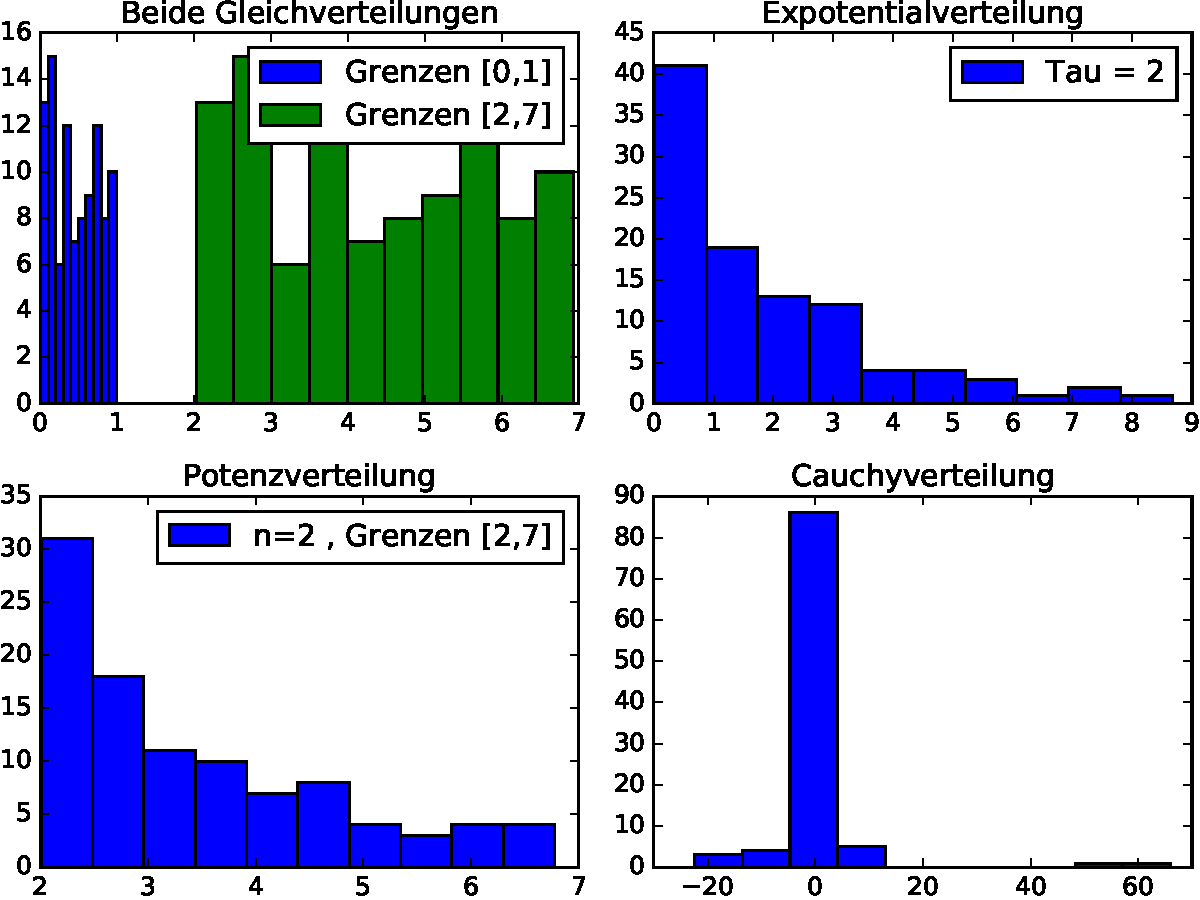
\includegraphics[height = 10cm]{plots/A1abcd.pdf}
  \caption{Diagramme zu den einzelnen Verteilungen.}
  \label{fig:A1abcd}
\end{figure}


\subsection{e)}
Eine Methode um aus diskreten Werten Zufallsvariablen zu generieren ist, zuerst eine 
kummulative Wahrscheinlichkeit für alle $x_k$ mit $k = 1, ... ,n$ zu berechnen, mit 
\begin{equation}
P_{k+1} = \sum_{i=1} ^{k} P(x_i) \quad \text{mit} \quad P_1 = 0 , \; P_{n+1} = 1 \; .
\end{equation}
Das wurde von uns in Python wie folgt implimentiert.

\lstinputlisting[language=Python, firstline=32, lastline=39]{plots/Aufgabe1.py}
Hier stellt \textit{wahrsch} die Wahrscheinlichkeit berechnet aus den Counts da und 
\textit{kumuwahr} die kummulative Wahrscheinlichkeit. Die for-Schleife führt eigentlich nur die 
Summe aus. 
Um nun die diskreten Zufallsvariablen zu bekommen nimmt man die gleichverteilten Zufallswerte $u$ 
und vergleicht diese mit den Elementen $P_{k-1} < u < P_k$ so erhält man den Index $k$ für den 
die Ungleichung erfüllt ist. Der Index ist dann auch der Index der diskreten Zufallsvariable 
anhand dem man die Zufallsvarable auslesen kann. In dem Fall hier ist es der Index eines 
\textit{binmid} Wertes. Die Inplementierung in Python folgt.
 
\lstinputlisting[language=Python, firstline=40, lastline=47]{plots/Aufgabe1.py}
Das Historgamm dazu ist in der Abbildung \ref{fig:A1eplot} dargestellt.
\begin{figure}
  \centering
  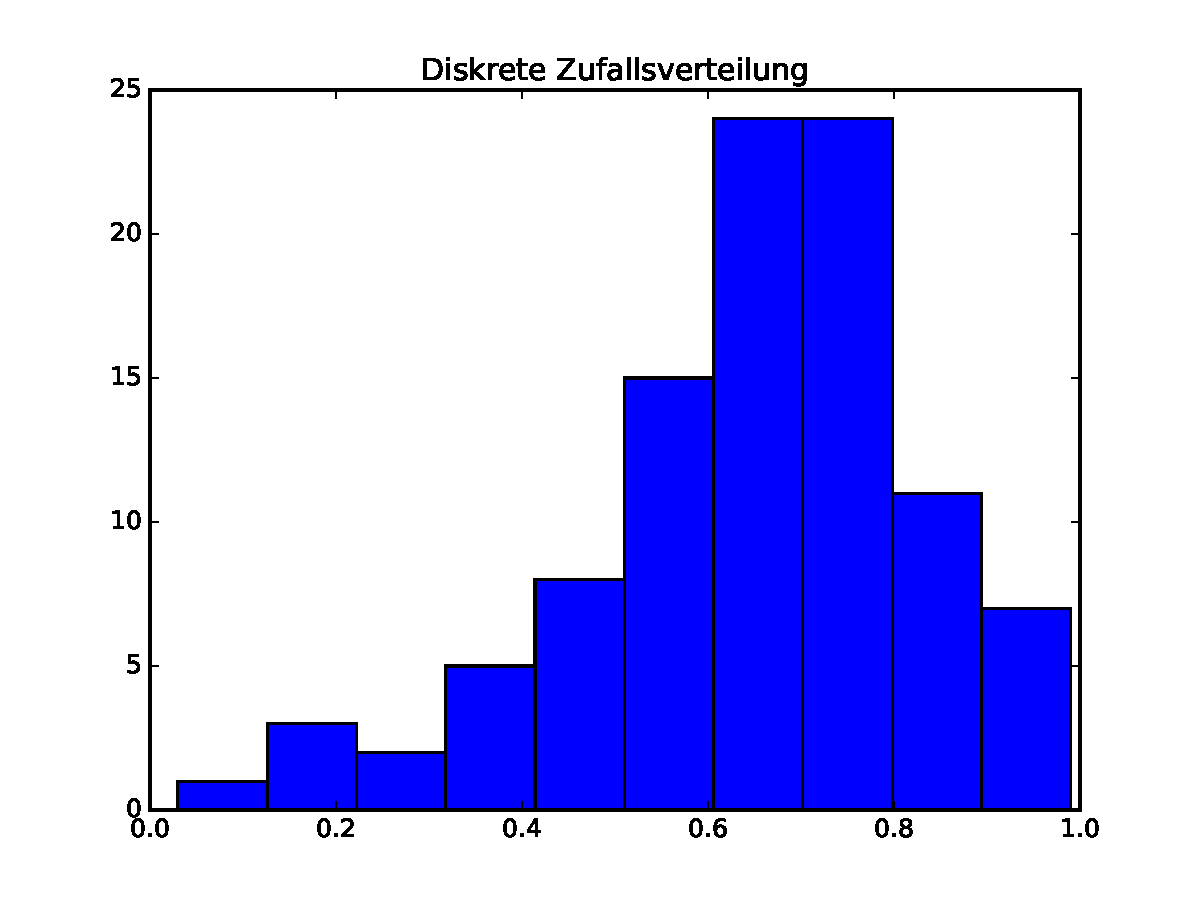
\includegraphics[height = 10cm]{plots/A1eplot.pdf}
  \caption{Histogramm zu den diskreten Zufallsvariablen.}
  \label{fig:A1eplot}
\end{figure}
 


\section{Aufgabe 2}
\label{sec:Aufgabe2}
\lstinputlisting[language=Python, firstline=15, lastline=21]{plots/plot.py}

\section{Aufgabe 3}

\label{sec:Aufgab3}
% \lstinputlisting[language=Python, firstline=15, lastline=21]{plots/plot.py}
\paragraph{a)}
Die Mittelwerte $\mu_{P0},\mu_{P1}$ wurden nach den Methoden der VL berechnet in Python wurde dies wie folgt
implimentiert:
\lstinputlisting[language=Python, firstline=12, lastline=24]{plots/Aufgabe3.py}
Dabei werden in den Zeilen 4 bis 9 nur jeweils die x und y Einträge in arrays geschrieben. Die Mittelwerte
dieser in ein 2D-array gesetzt ergeben die $\mu_{P0}= \texttt{mup0},\mu_{P1}=\texttt{mup1}$ Mittelwerte.
Der Mittelwert \texttt{mup001} ist für den Aufgabenteil h.
\paragraph{b)}
Die Kovarianzmatrizen wurden mit einer Numpy Funktion berechnet.
\lstinputlisting[language=Python, firstline=26, lastline=30]{plots/Aufgabe3.py}
Kovarianzmatrix Population 0:
\begin{equation}
\begin{pmatrix}
12.20892862& 8.15840984\\
8.15840984& 6.72286327
\end{pmatrix}
\end{equation}
Kovarianzmatrix Population 1:
\begin{equation}
\begin{pmatrix}
12.35218537 & 7.4107561\\4
 7.41075614 & 5.47731503
\end{pmatrix}
\end{equation}
Kovarianzmatrix Population 0 und 1:
\begin{equation}
\begin{pmatrix}
21.32208007 & 7.94257453\\
 7.94257453 & 6.1025583
\end{pmatrix}
\end{equation}
Kovarianzmatrix Population 0\_1000:
\begin{equation}
\begin{pmatrix}
12.23612255 & 8.16049883\\
 8.16049883 & 6.75819008
\end{pmatrix}
\end{equation}
Kovarianzmatrix Population 0 und 0\_1000:
\begin{equation}
\begin{pmatrix}
12.21067453 & 8.15842886\\
 8.15842886 & 6.72630542
\end{pmatrix}
\end{equation}
\paragraph{c)} \quad \newline
\lstinputlisting[language=Python, firstline=37, lastline=56]{plots/Aufgabe3.py}
In den Zeilen eins bis drei werden hier nur einmal die Populationen zusammengefasst. Darauf werden
die Streumatrizen wie aus der VL bestimmt (Zeilen 5-15). Die Lösung für die Fisher Diskriminante
ist aus der Vl bekannt und wird dann nur noch durch die gegebene Gleichung berechnet (Zeile 17).
Danach wird diese nur noch normiert. Das selbe (Zeile 17-20) wird für den Aufgabenteil h wiederholt.
Dann ergibt sich für die Population 0 und 1
\begin{equation}
\vec{\lambda} = \lambda \cdot
\begin{pmatrix}
-0.61886608\\
0.78549652
\end{pmatrix}
\end{equation}
und für die Population 0 und 0\_1000:
\begin{equation}
\vec{\lambda} = \lambda \cdot
\begin{pmatrix}
-0.46250292 \\
0.88661776
\end{pmatrix}
\end{equation}
\paragraph{d)}
Zur Berechnung der Projektion wurde folgende Funktion implimentiert:
\lstinputlisting[language=Python, firstline=67, lastline=68]{plots/Aufgabe3.py}
Die Histogramme sind in den Abbildungen \ref{fig:hist01} und \ref{fig:hist001} (Aufgabenteil h) zu sehen.
\begin{figure}
  \centering
  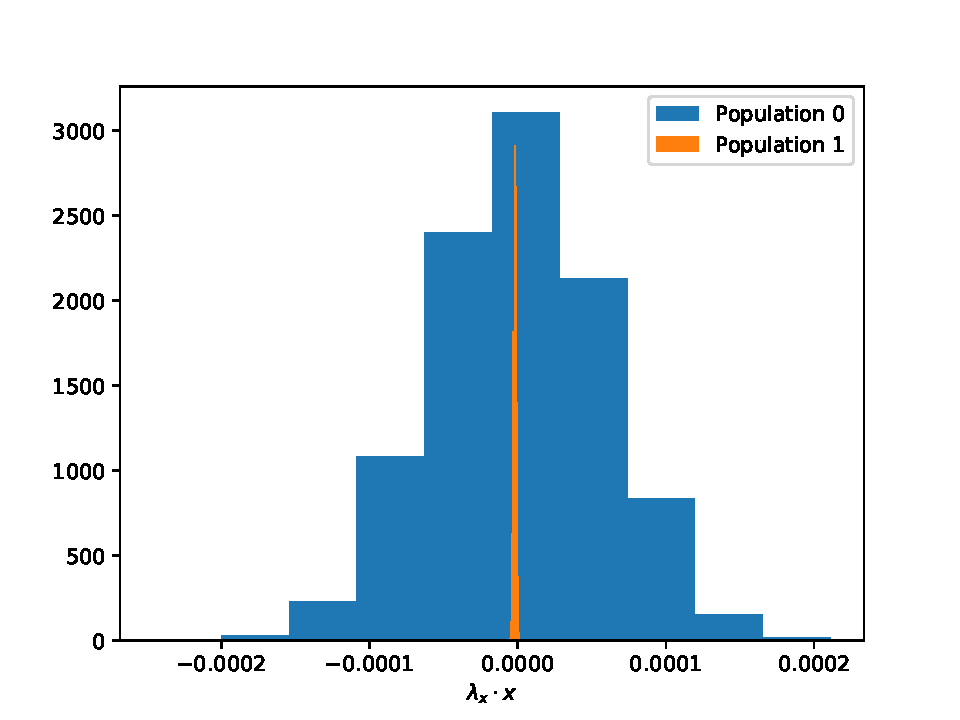
\includegraphics[height = 7cm]{plots/Projektion1dimhist.pdf}
  \caption{Projektion der Populationen 0 und 1.}
  \label{fig:hist01}
\end{figure}
\begin{figure}
  \centering
  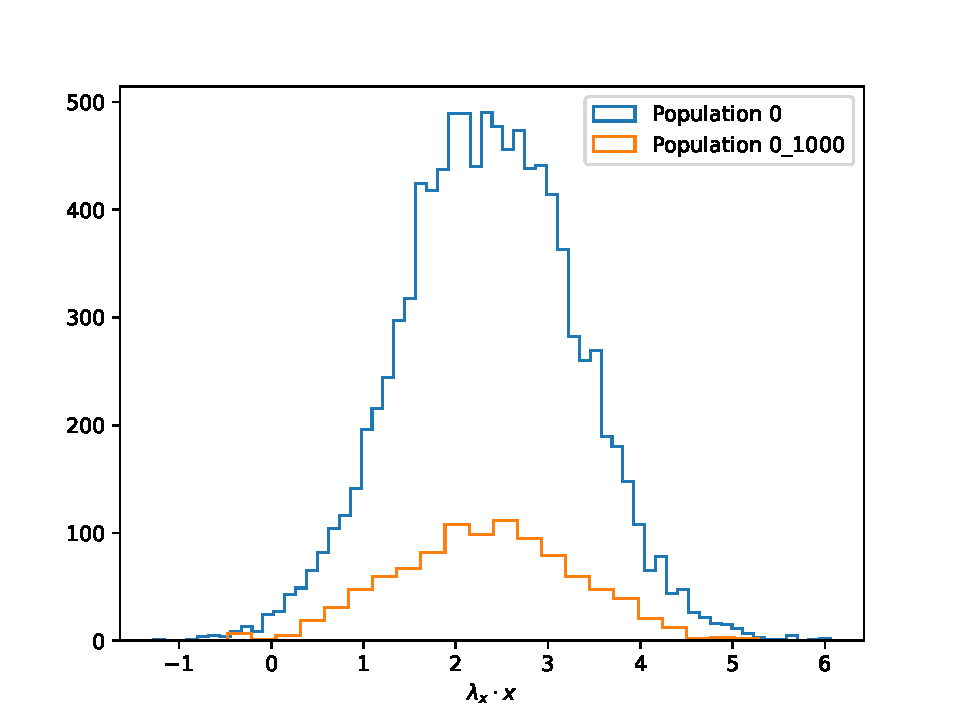
\includegraphics[height = 7cm]{plots/2Projektion1dimhist.pdf}
  \caption{Projektion der Populationen 0 und 0\_1000.}
  \label{fig:hist001}
\end{figure}
\FloatBarrier
\paragraph{e)}
Zur Bestimmung der Reinheit und Effizienz wurde folgende Funktion implimentiert:
\lstinputlisting[language=Python, firstline=86, lastline=102]{plots/Aufgabe3.py}
Die Ergebnisse sind in den Abbildungen \ref{fig:RE1} und \ref{fig:RE2} (AT h) dargestellt.
Gesuchte $\lambda_{Cut}$ Werte:
\begin{equation}
\lambda_{0\&1} = 2.13667347 \quad \text{und} \quad \lambda_{0\&0\_1} = 5.19070384	\; .
\end{equation}

\begin{figure}
  \centering
  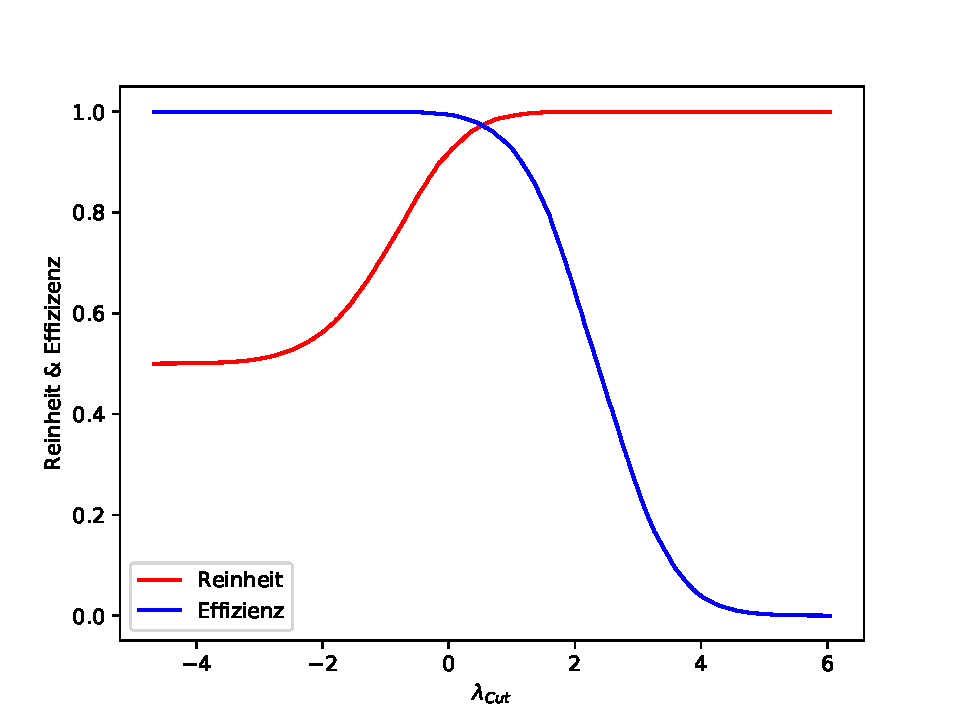
\includegraphics[height = 7cm]{plots/ReinheitEffizienzplot.pdf}
  \caption{Reinheit und Effizienz - Populationen 0 und 1.}
  \label{fig:RE1}
\end{figure}
\begin{figure}
  \centering
  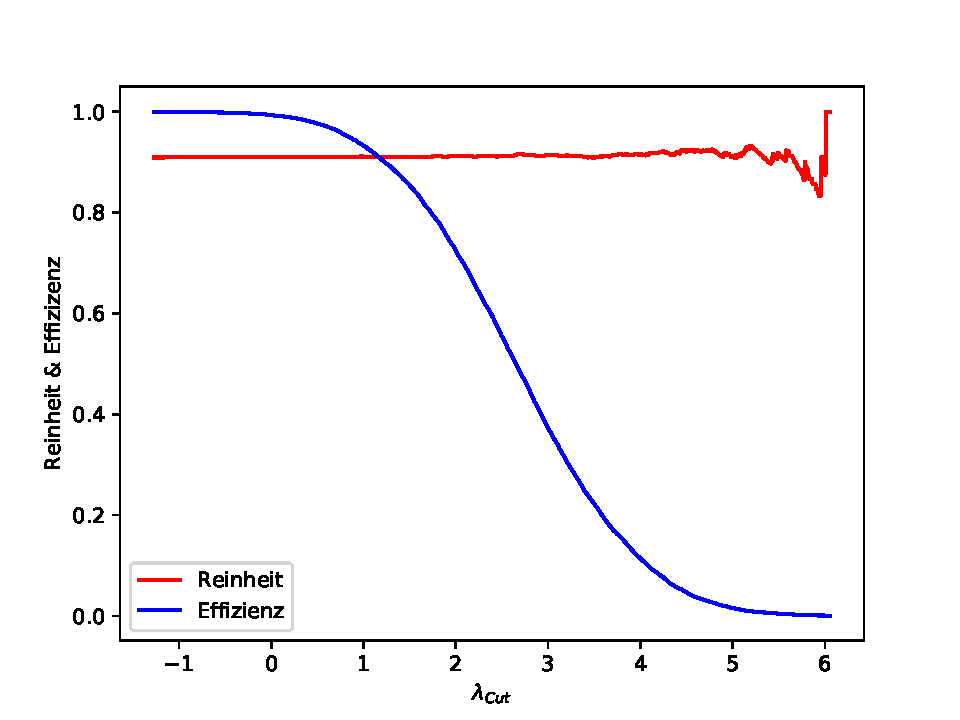
\includegraphics[height = 7cm]{plots/2ReinheitEffizienzplot.pdf}
  \caption{Reinheit und Effizienz - Populationen 0 und 0\_1000.}
  \label{fig:RE2}
\end{figure}
\FloatBarrier
\paragraph{f)}
Zur Berechnung des Signal-Untergrundverhältnisses nach der Trennung wurde folgende Funktion implimentiert.
\lstinputlisting[language=Python, firstline=125, lastline=134]{plots/Aufgabe3.py}
Die Ergebnisse sind in den Abbildungen \ref{fig:SB1} und \ref{fig:SB1} (AT h) dargestellt.
Gesuchte $\lambda_{Cut}$ Werte:
\begin{equation}
\lambda_{0\&1} = 0.52587484 \quad \text{und} \quad \lambda_{0\&0\_1} \approx -1.2 \; .
\end{equation}


\begin{figure}
  \centering
  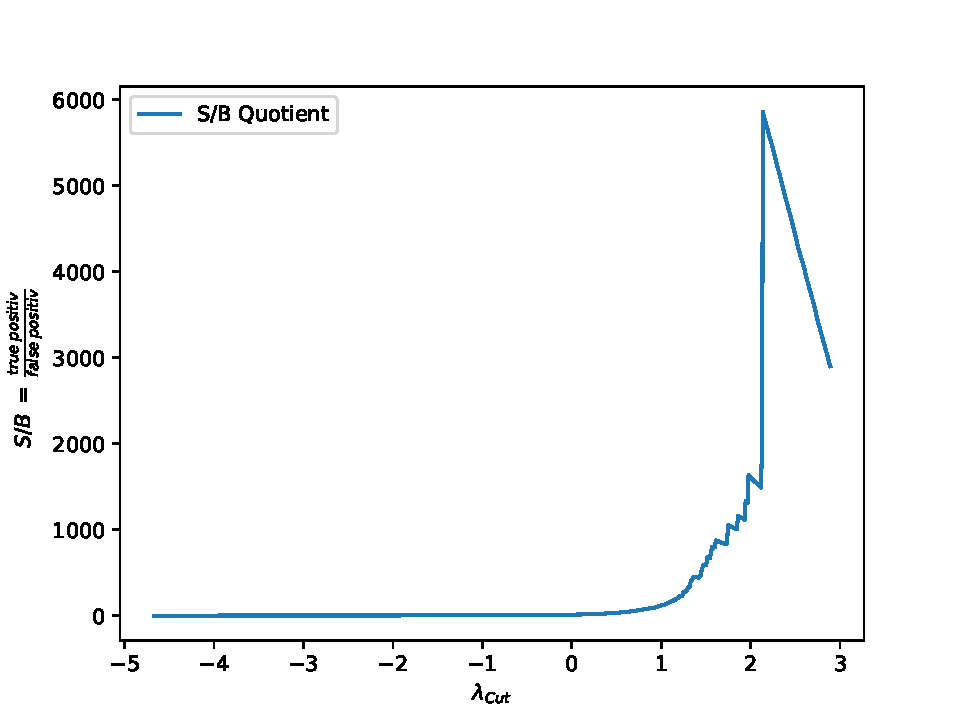
\includegraphics[height = 7cm]{plots/SBRatioplot.pdf}
  \caption{Signal-Untergrundverhältnisses für Populationen 0 und 1.}
  \label{fig:SB1}
\end{figure}
\begin{figure}
  \centering
  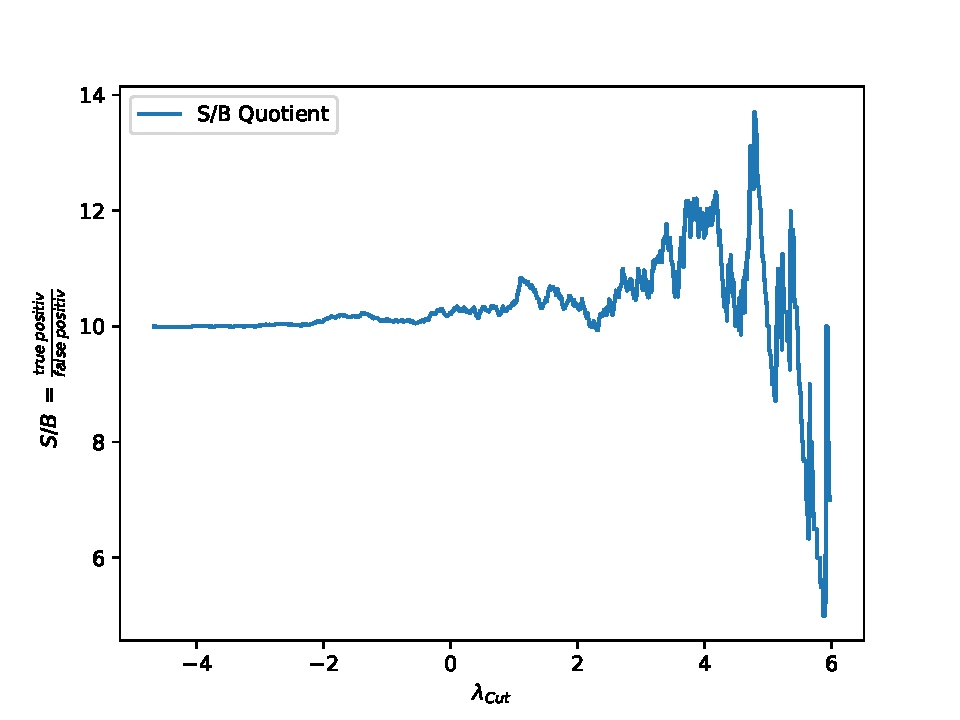
\includegraphics[height = 7cm]{plots/2SBRatioplot.pdf}
  \caption{Signal-Untergrundverhältnisses für Populationen 0 und 0\_1000.}
  \label{fig:SB2}
\end{figure}
\paragraph{g)}
Zur Berechnung der Signifikanz nach der Trennung wurde folgende Funktion implimentiert.
\lstinputlisting[language=Python, firstline=151, lastline=160]{plots/Aufgabe3.py}
Die Ergebnisse sind in den Abbildungen \ref{fig:S1} und \ref{fig:S2} (AT h) dargestellt.
\begin{figure}
  \centering
  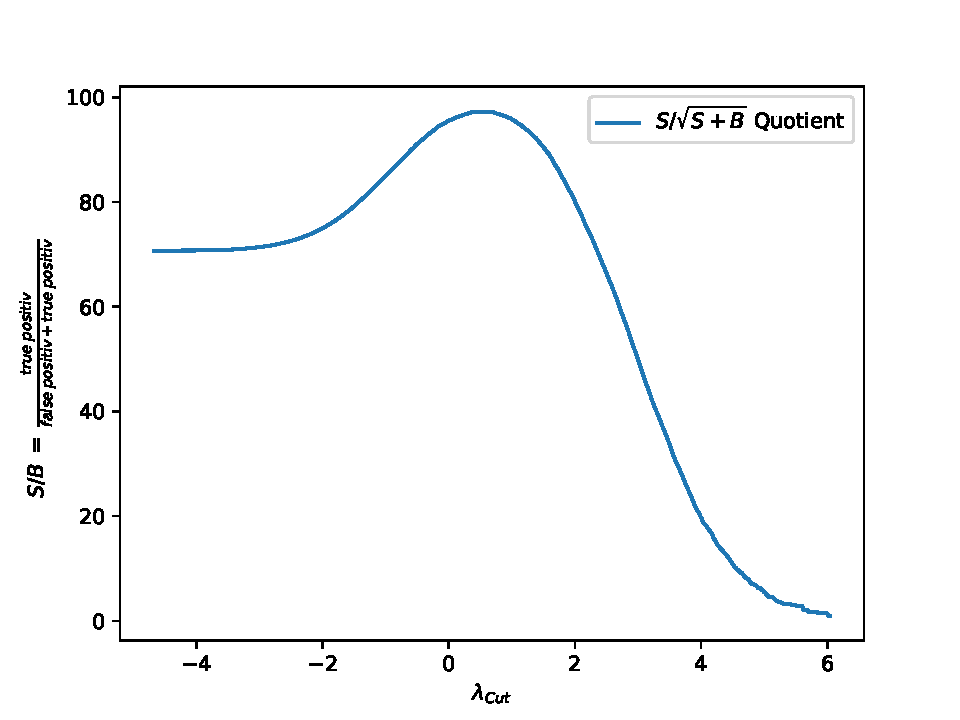
\includegraphics[height = 7cm]{plots/Signifikanzplot.pdf}
  \caption{Signifikanz nach der Trennung Populationen 0 und 1.}
  \label{fig:S1}
\end{figure}
\begin{figure}
  \centering
  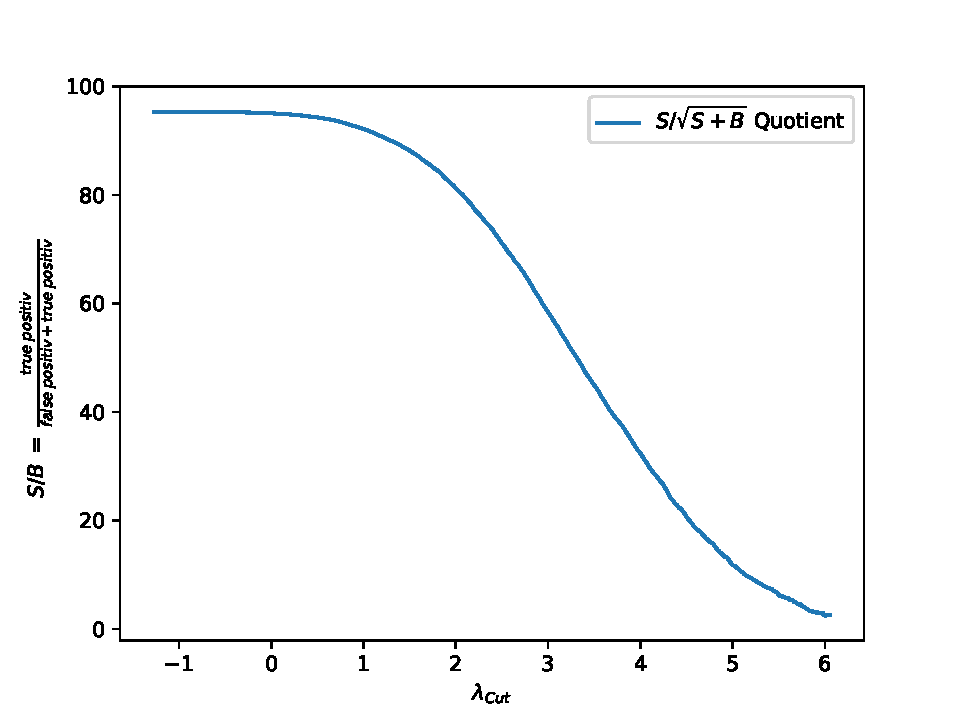
\includegraphics[height = 7cm]{plots/2Signifikanzplot.pdf}
  \caption{Signifikanz nach der Trennung Populationen 0 und 0\_1000.}
  \label{fig:S2}
\end{figure}
\FloatBarrier
\paragraph{d)} siehe oben

%\section{Aufgabe 4}
\label{sec:Aufgabe4}
\subsection{Teil a)}
Die Wahrscheinlichkeit, dass die Summe der Würfel 9 ist, lässt sich aus den verschiedenen Möglichkeiten den
erwünschten Wert 9 aus allen Ereignissen zu erhalen,
bestimmen. Insgesamt gibt es 36 mögliche Ereignisse. Mit zwei Würfeln lässt sich der Wert 9 nur mit den Kombinationen 3\&6 sowie 4\&5 erreichen.
Insgesamt gibt es also 4 Möglichkeiten, da es egal ist welcher der Würfel, welchen Wert hat.
Daraus folgt
\begin{equation*}
  P(W_{\symup{rot}} + W_{\symup{blau}} = 9) = \frac{4}{36} = \frac{1}{9} .
\end{equation*}
\subsection{Teil b)}
Um die Wahrscheinlichkeit zu bestimmen, eine Summe von 9 oder mehr zu erhalten,
werden die gewünschten Kombinationen abgezählt: 6\&3, 3\&6, 6\&4, 4\&6, 6\&5, 5\&6, 6\&6, 5\&4, 4\&5, 5\&5.
Es gibt also insgesamt 10 Möglichkeiten.
\begin{equation*}
  P(W_{\symup{rot}} + W_{\symup{blau}} \geq 9) = \frac{10}{36} = \frac{5}{18} .
\end{equation*}
\subsection{Teil c)}
Es gibt nur 2 Möglichkeiten, dass ein Würfel 4 und der andere 5 zeigt.
\begin{equation*}
  P(W_{\symup{blau/rot}} = 4, W_{\symup{blau/rot}} = 5) = \frac{2}{36} = \frac{1}{18} .
\end{equation*}
\subsection{Teil d)}
Es gibt genau eine Möglichkeit, dass der rote Würfel 4 und der blaue 5 zeigt.
\begin{equation*}
  P(W_{\symup{rot}} = 4, W_{\symup{blau}} = 5) = \frac{1}{36} .
\end{equation*}
\subsection{Teil e)}
Da bekannt ist, dass der rote Würfel eine 4 zeigt, bleiben noch 6 mögliche Ereignisse
für den blauen Würfel.
Dass die Summe 9 ist gilt also nur, wenn der blaue Würfel eine 5 zeigt.
\begin{equation*}
   P(W_{\symup{rot}} + W_{\symup{blau}} = 9 |W_{\symup{rot}} = 4) = P( W_{\symup{blau}} = 5) =  \frac{1}{6} .
\end{equation*}
\subsection{Teil f)}
Es gibt nur zwei Ereignisse, 5 und 6, die zusammen mit der roten 4 eine 9 ergeben:
\begin{equation*}
  P(W_{\symup{rot}} + W_{\symup{blau}} \geq 9 \ | \ W_{\symup{rot}} = 4) = \frac{2}{6} = \frac{1}{3}.
\end{equation*}
\subsection{Aufgabenteil g)}
Es gibt nur eine Möglichkeit, also gilt wie in Teil e) :
\begin{equation*}
  P(W_{\symup{rot}} = 4, \, W_{\symup{blau}} = 5 \ | \ W_{\symup{rot}} = 4) = \frac{1}{6}.
\end{equation*}


\printbibliography

\end{document}
